\chapter{Metaheuristics}

\section{What is a metaheuristic?}

A metaheuristic is a problem-solving strategy that consists in a set of steps with the purpose of finding good solutions to optimization problems.
Unlike heuristics, they are not dependent or tailored to a specific problem in particular, instead they are general problem-solving frameworks applicable to a wide range of cases.
While heuristics typically have very specific execution procedures, metaheuristics are generally more abstract, providing a broad approach to follow while leaving the details of implementation to the researcher.

They do not guarantee optimality but aim to efficiently find high-quality solutions.
For this reason, they often operate iteratively, repeating a set of steps for a specified number of iterations or until a termination condition is met.
Common termination conditions include achieving convergence in the objective function, finding a solution considered sufficiently good, or reaching a time limit.
The broad definition of metaheuristics also accounts for the frequent need to adjust parameters for optimization, which may vary across different implementations.
% This difference with the heuristics can be confirmed also by the ones that we explored in this work.

It's also worth mentioning the fact that heuristics like NN and EM are focused on discovering new solutions at each iteration, while metaheuristics usually start from an existing feasible solution, with the objective of improving it.
% Popular metaheuristics that we worked on are \textit{Simulated Annealing}, \textit{Genetic algorithm}, \textit{Tabu Search}, and \textit{Variable Neighborhood Search0}.

\section{2-Opt}

The 2-Opt metaheuristic is a local search method used to improve the solution in optimization problems.
It is based on the idea of iteratively improving a feasible solution of the problem by swapping pairs of edges creating a new solution.
The name itself comes from the fact it optimizes the solution by replacing a couple of edges at every iteration.

\begin{figure}[htbp]
    \centering
    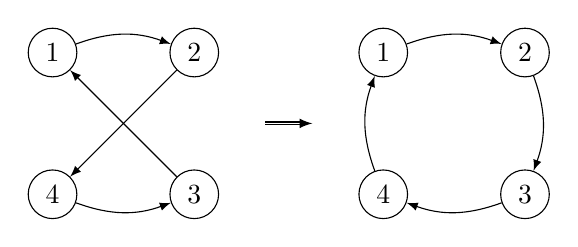
\begin{tikzpicture}[scale=0.6]
        \node[circle, draw, fill=white] (A0) at (0, 0) {1};
        \node[circle, draw, fill=white] (B0) at (3, 0) {2};
        \node[circle, draw, fill=white] (C0) at (3, -3) {3};
        \node[circle, draw, fill=white] (D0) at (0, -3) {4};
    
        \draw[-latex] (A0) to[bend left=20] (B0);
        \draw[-latex] (B0) -- (D0);
        \draw[-latex] (D0) to[bend right=20] (C0);
        \draw[-latex] (C0) -- (A0);
    
        \draw[double,-latex] (4.5,-1.5) -- (5.5,-1.5);
    
        \node[circle, draw, fill=white] (A1) at (7, 0) {1};
        \node[circle, draw, fill=white] (B1) at (10, 0) {2};
        \node[circle, draw, fill=white] (C1) at (10, -3) {3};
        \node[circle, draw, fill=white] (D1) at (7, -3) {4};
    
        \draw[-latex] (A1) to[bend left=20] (B1);
        \draw[-latex] (B1) to[bend left=20] (C1);
        \draw[-latex] (C1) to[bend left=20] (D1);
        \draw[-latex] (D1) to[bend left=20] (A1);
    \end{tikzpicture}
    \caption{Representation of an edge swap in 2-Opt.}
    \label{fig:2optMoves}
\end{figure}

A \textbf{swap} is a simple computation in which two edges are removed from a solution and replaced with a new pair of edges such that the newly obtained tour is a feasible solution.
Every swap is characterized by their \textbf{offset value}, which represent the quality of the swap and is calculated as the sum of the edges added minus the sum of the edges removed.
An offset is considered an optimizing offset only if its value is negative.
Each solution usually allows for a finite yet very large number of swaps, however 2-Opt only involves swaps that reduce the overall cost of the tour, or a swaps with an optimizing offset.
These swaps are referred to as \textbf{optimizing swaps} or \textbf{2-Opt moves}.

The key step in the 2-Opt algorithm consists in finding and choosing a combination of edges that allows for a 2-Opt move.
A simple approach consists in scanning all possible swaps and choose the first detected optimizing move.
Another approach consists in scanning all possible swaps like before, and selecting the swap with the best offset.
The first procedure has the advantage of being able to find a suitable swap faster, while the quality of the optimizing swaps is never considered.
As opposed to the first method, the second procedure takes longer to find swaps, but the swap selected is the one that reduces the cost of the solution the most.
In this project we implemented the second approach.

%Once the edges are swapped the total cost of the tour is recalculated, and if it is lower than the previous cost, the swap is integrated in the solution permanently, or until a better swap involving one of those two edges is found.
%This operation is iterated across all possible pairs of the tour, and is repeated until a time limit is reached, or no further improvements are possible (which involves checking all possible combinations many time, making it infeasible for real-life complex scenarios).
2-Opt can improve significantly a solution, while maintaining an acceptable computational complexity across the board.
Each iteration of 2-Opt is of $O(n^2)$ complexity, while the number of iterations depends both on the size and quality of the starting solution.
Its main limitation is the fact that due of it being a local search method, it usually gets stuck in a local minima, thus failing to find the best solution.

\begin{figure}[htbp]
    \textbf{2-Opt} \\
    \begin{algorithm}[H]
        \SetKwInOut{Input}{Input}
        % \SetKwInOut{Output}{Output}
        \Input{Graph $G(V,E)$ \newline Cost function $C: E \rightarrow \mathbb{R}$, where $c_{i,j} = C(e_{i,j})$ \newline A tour $T$ of $G$}
        % \Output{A better or equaly quality solution}
        \BlankLine
        %$finished \gets 0$ \\
        \While{true}{%$finished = 0$}{
            $s \gets$ swap with the lowest offset currently in $T$\\
            \eIf{offset($s$) $<$ 0}{
                apply $s$ to $T$
            }{
                break%$finished \gets 1$
            }
        }
    \end{algorithm}
    \caption{2-Opt algorithm} \label{fig:2OptPseudocode}
\end{figure}

\subsection{Implementation}

While in the Cost-Matrix approach the implementation is exactly the same as \figurename{ \ref{fig:2OptPseudocode}}, the same cannot be said for the other approaches.
As we saw in the previous chapter, the Base and AVX methods can be enhanced by using approximation techniques.

The function which finds the 2-Opt move with the lowest offset value is presented in two versions: one which computed the exact edge cost and another which uses approximations in the edge cost computation.
This is mandatory since by only using the approximated search some optimizing swaps might be missed, which is especially true when the offset of those swaps is close to zero.
Therefore an easy fix is to use the approximated search as long as the selected swap is optimizing when recomputed with the accurate methods.
Recomputing the offset at the proposal of any 2-Opt move is necessary, since the approximations might cause an unoptimizing swap to look like an optimizing one.

\begin{figure}[htbp]
    \textbf{2-Opt with approximated seach} \\
    \begin{algorithm}[H]
        \SetKwInOut{Input}{Input}
        % \SetKwInOut{Output}{Output}
        \Input{Graph $G(V,E)$ \newline Cost function $C: E \rightarrow \mathbb{R}$, where $c_{i,j} = C(e_{i,j})$ \newline A tour $T$ of $G$}
        % \Output{A better or equaly quality solution}
        \BlankLine
        $useApprox \gets$ True \\
        \While{true}{%$finished = 0$}{
            \eIf{useApprox}{
                $s \gets$ swap with the lowest offset currently in $T$ w.r.t. cost approximations \\
                recompute offset of $s$ using accurate cost functions
            }{
                $s \gets$ swap with the lowest offset currently in $T$
            }
            \eIf{offset($s$) $<$ 0}{
                apply $s$ to $T$
            }{
                \eIf{useApprox}{
                    $useApprox \gets$ False
                }{
                    break
                }
            }
        }
    \end{algorithm}
    \caption{2-Opt algorithm} \label{fig:2OptPseudocodeApprox}
\end{figure}

% % In our implementation of 2-opt we decided to optimize heavily the method using AVX functions rather than multithreading 
% % (NOTE: check, and why AVX).
% The function that takes care of the application of the metaheuristic is apply2OptBestFix, to which we pass the solution to refine, and will apply the options selected at launch. 
% The heart of the algorithm lies in the two specular functions \_2OptBestFix and \_2OptBestFixApprox.
% The former will compute the exact edge cost when evaluating edge swaps, considering the actual distance between the points and delivering a more precise result, with the cost of a slower computation, especially for larger instances.
% The latter uses an approximated computation of the edges cost and provides a faster iteration time, with the counterpart of possibly producing slightly worse solutions. 
% These two methods will iterate over all possible pairs of edges in the tour and compute the potential decrease in total tour length if we were to apply the swap.
% The data regarding the best swap found so far, offset of the cost and the edges, is kept in the bestFix struct, to which we will compare each potential swap and which will be then implemented at the end of the iteration.


\subsection{3-Opt}

The 3-Opt metaheuristic is an extension of the 2-Opt algorithm, with the key difference that it is not limited to swaps involving just two edges, but instead considers swaps of up to three edges. This broader approach allows for a larger neighborhood of solutions to be explored, potentially enabling the algorithm to escape local minima that 2-Opt might not be able to overcome.

It is important to note, however, that while the solution space is expanded, escaping all local minima is not guaranteed and is generally not achievable with algorithms like this. The overall process is similar to 2-Opt, with the primary distinction being the number of nodes involved in each swap and the various configurations that these swaps can take.

The concepts of \textbf{swap}, \textbf{optimizing swap} and \textbf{offset value} remain the same as in the 2-Opt method, but they are extended to include three edges.
As shown in \figurename{ \ref{fig:3optMoves}}, the number of possible edge swaps increases significantly.
This not only raises the computational complexity due to the greater number of three-edge configurations, but also increases the asymptotic factor, which changes to $O(n^3)$ per iteration.

% As shown in figure \ref{fig:3optMoves}, starting from an existing solution, we iteratively consider three edges instead of two, and we change the way they are connected, looking for the one that has lower total cost.
% If a combination is found to improve the total cost of the solution then the swap is implemented, otherwise a different set of three edges is taken into consideration.
% Just as for 2-opt this iterative process can continue until a time limit is reached or until no more improving moves are possible.

\begin{figure}[htbp]
    \centering
    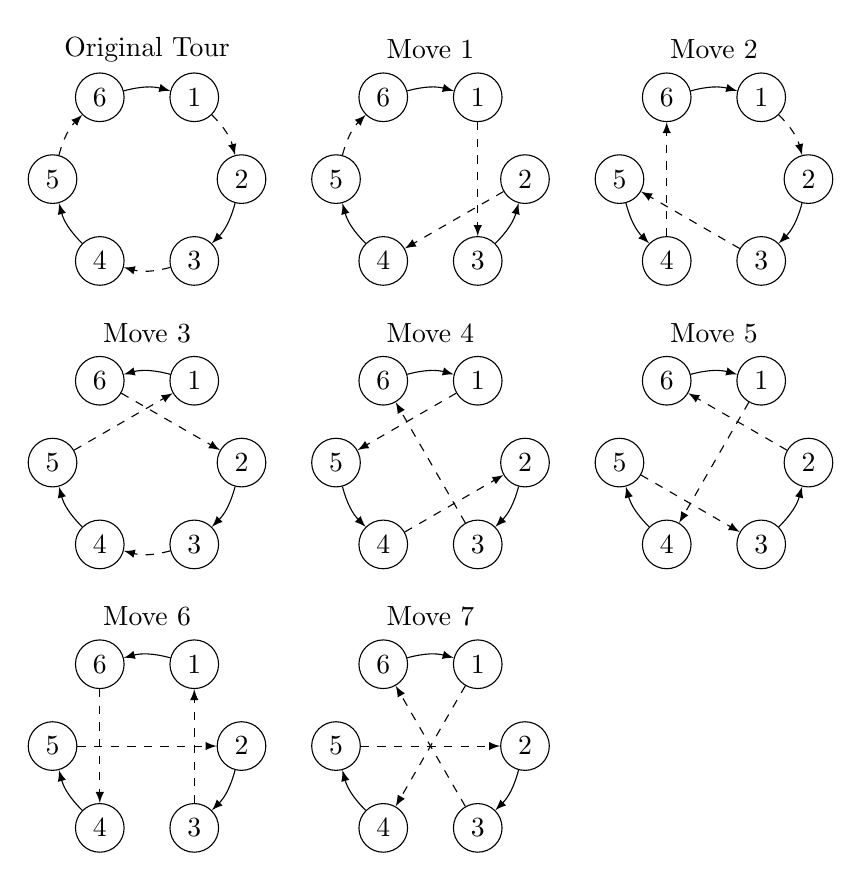
\begin{tikzpicture}[scale=0.6]
        \begin{scope}[shift={(0, 0)}]
            \node at (0, 2.75) {Original Tour};
        
            \node[circle, draw, fill=white] (N1) at ({60 * 2}:2) {6};
            \node[circle, draw, fill=white] (N2) at ({60 * 1}:2) {1};
            \node[circle, draw, fill=white] (N3) at ({60 * 0}:2) {2};
            \node[circle, draw, fill=white] (N4) at ({60 * 5}:2) {3};
            \node[circle, draw, fill=white] (N5) at ({60 * 4}:2) {4};
            \node[circle, draw, fill=white] (N6) at ({60 * 3}:2) {5};
        
            \draw[-latex] (N1) to[bend left=15] (N2);
            \draw[-latex,dashed] (N2) to[bend left=15] (N3);
            \draw[-latex] (N3) to[bend left=15] (N4);
            \draw[-latex,dashed] (N4) to[bend left=15] (N5);
            \draw[-latex] (N5) to[bend left=15] (N6);
            \draw[-latex,dashed] (N6) to[bend left=15] (N1);
        \end{scope}
    
        \begin{scope}[shift={(6, 0)}]
            \node at (0, 2.75) {Move 1};
        
            \node[circle, draw, fill=white] (N1) at ({60 * 2}:2) {6};
            \node[circle, draw, fill=white] (N2) at ({60 * 1}:2) {1};
            \node[circle, draw, fill=white] (N3) at ({60 * 0}:2) {2};
            \node[circle, draw, fill=white] (N4) at ({60 * 5}:2) {3};
            \node[circle, draw, fill=white] (N5) at ({60 * 4}:2) {4};
            \node[circle, draw, fill=white] (N6) at ({60 * 3}:2) {5};
        
            \draw[-latex] (N1) to[bend left=15] (N2);
            \draw[-latex,dashed] (N2) to (N4);
            \draw[-latex,dashed] (N3) to (N5);
            \draw[-latex] (N4) to[bend right=15] (N3);
            \draw[-latex] (N5) to[bend left=15] (N6);
            \draw[-latex,dashed] (N6) to[bend left=15] (N1);
        \end{scope}
    
        \begin{scope}[shift={(12, 0)}]
            \node at (0, 2.75) {Move 2};
        
            \node[circle, draw, fill=white] (N1) at ({60 * 2}:2) {6};
            \node[circle, draw, fill=white] (N2) at ({60 * 1}:2) {1};
            \node[circle, draw, fill=white] (N3) at ({60 * 0}:2) {2};
            \node[circle, draw, fill=white] (N4) at ({60 * 5}:2) {3};
            \node[circle, draw, fill=white] (N5) at ({60 * 4}:2) {4};
            \node[circle, draw, fill=white] (N6) at ({60 * 3}:2) {5};
        
            \draw[-latex] (N1) to[bend left=15] (N2);
            \draw[-latex,dashed] (N2) to[bend left=15] (N3);
            \draw[-latex] (N3) to[bend left=15] (N4);
            \draw[-latex,dashed] (N4) to (N6);
            \draw[-latex,dashed] (N5) to (N1);
            \draw[-latex] (N6) to[bend right=15] (N5);
        \end{scope}
    
        \begin{scope}[shift={(0, -6)}]
            \node at (0, 2.75) {Move 3};
        
            \node[circle, draw, fill=white] (N1) at ({60 * 2}:2) {6};
            \node[circle, draw, fill=white] (N2) at ({60 * 1}:2) {1};
            \node[circle, draw, fill=white] (N3) at ({60 * 0}:2) {2};
            \node[circle, draw, fill=white] (N4) at ({60 * 5}:2) {3};
            \node[circle, draw, fill=white] (N5) at ({60 * 4}:2) {4};
            \node[circle, draw, fill=white] (N6) at ({60 * 3}:2) {5};
        
            \draw[-latex,dashed] (N1) to (N3);
            \draw[-latex] (N2) to[bend right=15] (N1);
            \draw[-latex] (N3) to[bend left=15] (N4);
            \draw[-latex,dashed] (N4) to[bend left=15] (N5);
            \draw[-latex] (N5) to[bend left=15] (N6);
            \draw[-latex,dashed] (N6) to (N2);
        \end{scope}
    
        \begin{scope}[shift={(6, -6)}]
            \node at (0, 2.75) {Move 4};
        
            \node[circle, draw, fill=white] (N1) at ({60 * 2}:2) {6};
            \node[circle, draw, fill=white] (N2) at ({60 * 1}:2) {1};
            \node[circle, draw, fill=white] (N3) at ({60 * 0}:2) {2};
            \node[circle, draw, fill=white] (N4) at ({60 * 5}:2) {3};
            \node[circle, draw, fill=white] (N5) at ({60 * 4}:2) {4};
            \node[circle, draw, fill=white] (N6) at ({60 * 3}:2) {5};
        
            \draw[-latex] (N1) to[bend left=15] (N2);
            \draw[-latex,dashed] (N2) to (N6);
            \draw[-latex] (N3) to[bend left=15] (N4);
            \draw[-latex,dashed] (N4) to (N1);
            \draw[-latex,dashed] (N5) to (N3);
            \draw[-latex] (N6) to[bend right=15] (N5);
        \end{scope}
    
        \begin{scope}[shift={(12, -6)}]
            \node at (0, 2.75) {Move 5};
        
            \node[circle, draw, fill=white] (N1) at ({60 * 2}:2) {6};
            \node[circle, draw, fill=white] (N2) at ({60 * 1}:2) {1};
            \node[circle, draw, fill=white] (N3) at ({60 * 0}:2) {2};
            \node[circle, draw, fill=white] (N4) at ({60 * 5}:2) {3};
            \node[circle, draw, fill=white] (N5) at ({60 * 4}:2) {4};
            \node[circle, draw, fill=white] (N6) at ({60 * 3}:2) {5};
        
            \draw[-latex] (N1) to[bend left=15] (N2);
            \draw[-latex,dashed] (N2) to (N5);
            \draw[-latex,dashed] (N3) to (N1);
            \draw[-latex] (N4) to[bend right=15] (N3);
            \draw[-latex] (N5) to[bend left=15] (N6);
            \draw[-latex,dashed] (N6) to (N4);
        \end{scope}
    
        \begin{scope}[shift={(0, -12)}]
            \node at (0, 2.75) {Move 6};
        
            \node[circle, draw, fill=white] (N1) at ({60 * 2}:2) {6};
            \node[circle, draw, fill=white] (N2) at ({60 * 1}:2) {1};
            \node[circle, draw, fill=white] (N3) at ({60 * 0}:2) {2};
            \node[circle, draw, fill=white] (N4) at ({60 * 5}:2) {3};
            \node[circle, draw, fill=white] (N5) at ({60 * 4}:2) {4};
            \node[circle, draw, fill=white] (N6) at ({60 * 3}:2) {5};
        
            \draw[-latex,dashed] (N1) to (N5);
            \draw[-latex] (N2) to[bend right=15] (N1);
            \draw[-latex] (N3) to[bend left=15] (N4);
            \draw[-latex,dashed] (N4) to (N2);
            \draw[-latex] (N5) to[bend left=15] (N6);
            \draw[-latex,dashed] (N6) to (N3);
        \end{scope}
    
        \begin{scope}[shift={(6, -12)}]
            \node at (0, 2.75) {Move 7};
        
            \node[circle, draw, fill=white] (N1) at ({60 * 2}:2) {6};
            \node[circle, draw, fill=white] (N2) at ({60 * 1}:2) {1};
            \node[circle, draw, fill=white] (N3) at ({60 * 0}:2) {2};
            \node[circle, draw, fill=white] (N4) at ({60 * 5}:2) {3};
            \node[circle, draw, fill=white] (N5) at ({60 * 4}:2) {4};
            \node[circle, draw, fill=white] (N6) at ({60 * 3}:2) {5};
        
            \draw[-latex] (N1) to[bend left=15] (N2);
            \draw[-latex,dashed] (N2) to (N5);
            \draw[-latex] (N3) to[bend left=15] (N4);
            \draw[-latex,dashed] (N4) to (N1);
            \draw[-latex] (N5) to[bend left=15] (N6);
            \draw[-latex,dashed] (N6) to (N3);
        \end{scope}
    
    \end{tikzpicture}
    \caption{3-Opt available moves}
    \label{fig:3optMoves}
\end{figure}

\subsection{Performance}

As expected, the quality of the solutions found by the 3-Opt algorithm consistently surpasses that of 2-Opt.
However, the time required by the two algorithms differs significantly: while 2-Opt completes the optimization of a NN generated solution in under a second, the 3-Opt algorithm takes over a minute to fully optimize the same solution.

\begin{figure}[htbp]
	\centering
	\begin{tikzpicture}
        \begin{axis}[
            xlabel={Cost Ratio},
            xmin=1, xmax=1.082,
            ymin=0, ymax=70,
            xtick={},
            ytick=\empty,
            legend style={at={(0.98,0.02)},anchor=south east,legend columns=1},
			legend cell align={left},
            %ymajorgrids=true,
            xmajorgrids=true,
            grid style=dashed,
        ]
        
        \addplot[Blue,mark=square,mark size=1.5] table[x=ones,y=idx, col sep=semicolon] {csv/23opt.csv}; 
        \addplot[Red,mark=o,mark size=1.5] table[x=2opt,y=idx, col sep=semicolon] {csv/23opt.csv};
        \addplot[Green,mark=triangle,mark size=1.5] table[x=3opt,y=idx, col sep=semicolon] {csv/23opt.csv}; 
        \addlegendentry{Optimal} 
        \addlegendentry{2-Opt}
        \addlegendentry{3-Opt}
            
        \end{axis}
    \end{tikzpicture}
	\caption{Performance comparison between different tenure sizes} \label{fig:23OptPerformance}
\end{figure}

\section{Tabu Search}

Tabu search is a metaheuristic designed to escape local minima.
The key idea is to avoid revisiting solutions that are known not to lead to the global optimum.

Let's assume we already have a refined solution and have reached a local minimum using the 2-Opt algorithm; we'll call this solution $x_k$.
Attempting to refine it further will not yield any improvement, as $x_k$ contains no 2-Opt moves, having been fully optimized by 2-Opt.
Tabu Search addresses this situation by accepting a \textit{bad} move; in other words, it performs a swap even if it results in a positive offset\footnote{A swap with a positive offset is a swap that increases the overall cost of the solution}.

Therefore, a new tour, $x_{k+1}$, is produced in the hope that applying 2-Opt again will yield a better solution than $x_k$.
However, there's a significant chance that the local search algorithm will revert from $x_{k+1}$ back to $x_k$, ending up in the same local minimum.
To avoid this, Tabu Seach uses a list called \textbf{tenure} which records the swaps made to escape a local minima.
This tenure list acts as a set of \textit{forbidden swaps}, ensuring that 2-Opt cannot perform swaps that are included in this data structure.

There are additional considerations regarding the tenure, particularly its size and contents.
Intuitively, the size of this list should be limited, otherwise, it might block too many edges, causing the optimization to become stuck with no swaps allowed.
This particular aspect of the tenure will be explored in the next subsection, in which multiple tenure sizes will be compared.
When the list is full, newly introduced \textit{forbidden swaps} replace the oldest elements in the tenure.

Another potential improvement regards a detection mechanism on whether the local minima has been escaped or not: by checking if 2-Opt made any improvements on the solution, even while avoiding \textit{forbidden moves}, it is possible to have a rough estimation on wether or not the local optima point has been escaped or not.
Upon detecting a potential escape, removing the oldest element from the tenure in hope of having actually escaped of the local minima.
% This size is called \textit{NOT TENURE}, and could be a fixed amount or it could be adaptive depending on the instance of the problem we are approaching.
% When the list is full, we start replacing the edges in it starting from the older ones.

It's imperative for this procedure to work to its fullest to always keep a copy of the best solution found throughout its execution between all working threads.
This process continues until some termination condition is reached.
As for the other metaheuristic presented in this project, the termination condition is a time limit.

\subsection{Edge locking implementation}

The mechanism in which \textit{forbidden swaps} are avoided can be difficult in its design.
In this project, we implemented the \textit{forbidden swaps} by preventing a single edge of such swaps from being used in a 2-Opt move.
We refer to this as the \textbf{edge locking procedure}.
For each \textit{forbidden swap} we lock in place a single edge, which is chosed at random between the two edges introduced by the swap.
Locking both edges will effectively prevent any improvement from any 2-Opt implementation, since the remaining part of the solution in already optimized.

In our implementation 2-Opt is an external method called from the tabu function, and we needed to figure out a way to prevent it to perform swaps which involve edges locked in the tenure.
To this end we exploited the cost cache implementation by setting the cost of locked edges to $-\infty$.

Let's consider a swap $s$ involving two \textit{current} edges, $e_{a,b}$, $e_{c,d}$, which are part of the current solution, and two \textit{alternative} edges, $e_{a,c}$, $e_{b,d}$, which are the edges that would replace $e_{a,b}$ and $e_{c,d}$.
The offset of $s$ is defined as
\[
    \text{offset}(s) = [c(e_{a,c}) + c(e_{b,d})] - [c(e_{a,b}) + c(e_{c,d})]
\]
In 2-Opt $s$ has a chance of being applied to a solution only if offset$(s)<0$.
If $e_{a,b}$ is a locked edge than $c(e_{a,b})=-\infty$, as defined in the cost cache.
This means that offset$(s) = [c(e_{a,c}) + c(e_{b,d})] - [-\infty + c(e_{c,d})] = \infty > 0$, so swap $s$ will not be applied by 2-Opt.
The same reasoning applies if $e_{c,d}$ is the locked edge.

Therefore we can apply the 2-Opt procedure in a way which respects the locked edges without any additional effort.
This edge locking mechanic can be used if 3-Opt is used as local search method instead, altough it is not guaranteed to be as effective.

\begin{figure}[htbp]
    \textbf{Tabu Search} \\
    \begin{algorithm}[H]
        \SetKwInOut{Input}{Input}
        \SetKwInOut{Output}{Output}
        \Input{Graph $G(V,E)$ \newline Cost function $c$ \newline A tour $T$ of $G$ \newline Size of the tenure $l_{size}$}
        \Output{A tour $T_{best}$ where $c(T_{best}) \leq c(T)$}
        \BlankLine
        $L \gets [\;]$\\
        $T \gets$ 2-Opt($T$)\\
        $T_{best} \gets T$\\
        \While{time limit is not reached}{
            \BlankLine
            select at random edges $e_0, e_1 \in T$ that are suitable to perform a swap in $T$\\
            \lIf{random$\{0,1\}$ = 1}{
                $e_0 \leftrightarrows e_1$
            }
            $L \gets L \cup \{e_0\}$\\
            \lIf{$|L| > l_{size}$}{
                $L \gets L \backslash \{l_0\}$, where $l_0$ is the oldest element in $L$
            }
            \BlankLine
            $T_{new} \gets$ 2-Opt($T$)\\
            \While{$c(T_{new}) \neq c(T)$}{
                $T \gets T_{new}$\\
                \lIf{$c(T) < c(T')$}{$T' \gets T$}
                $L \gets L \backslash \{l_0\}$\\
                $T_{new} \gets$ 2-Opt($T$)
            }
        }
        \Return $T_{best}$
    \end{algorithm}
    \caption{Tabu Search algorithm, where the Cost-cache related part are implicit as they are performed according to the tenure $L$} \label{fig:tabuPseudocode}
\end{figure}

% \subsection{Implementation}
% TabuSearch is the main method that manages the execution of the tabu algorithm.
% After receiving the solution, it sets the tenure size, which is implemented as an array of struct Edge, accordingly to input.
% We implemented a check on the value passed for this parameter: if we don't receive any specific size the default value of 2 is set; if we receive a value that is larger of equal to the amount of nodes in 
% the instace an error is thrown, since this will lead to the algorithm getting stuck; and lastly, if the value is larger than the 97\% of the 
% number of nodes a warning message will indicate the possibility of the method getting stuck and not respecting the time limit.
% After this, the function runTabu is launched whithin the threads and takes care of the execution of the metaheuristic, starting from the current best solution (CHECK IF ITS THE PASSED SOLUTION).
% The main loop that keeps going until the time limit consists in selecting two random edges in the solution, swapping them and locking one of the two by inserting it into the tenure.
% Once we have done that 2-opt is launched to refine the solution, and we keep relaunching it until there are no further improving moves possible, freeing the oldest element in the tenure before relaunching it every time.
% A counter is implemented to keep track of the number of iteration in which the method does not find a solution 
% that is better than the best one found so far, and when it reaches a threshold the working solution of the thread is resetted back to the best one.

\subsection{Performance}

To study the performance of the Tabu Search algorithm we implemented we must first choose a key hyperparameter: the \textbf{tenure size}.
We chose three different values which are compared in \figurename{ \ref{fig:tabuParmTune}}.

\begin{figure}[htbp]
	\centering
	\begin{tikzpicture}
        \begin{axis}[
            xlabel={Cost Ratio},
            %ylabel={Iterations/s Ratio},
            xmin=1, xmax=1.03,
            ymin=0, ymax=74,
            xtick={},
            ytick=\empty,
            legend style={at={(0.98,0.02)},anchor=south east,legend columns=1},
			legend cell align={left},
            %ymajorgrids=true,
            xmajorgrids=true,
            grid style=dashed,
        ]
        
        \addplot[Blue,mark=square,mark size=1.5] table[x=p1cost,y=idx, col sep=semicolon] {csv/tabu.csv}; 
        \addplot[Red,mark=o,mark size=1.5] table[x=p2cost,y=idx, col sep=semicolon] {csv/tabu.csv};
        \addplot[Green,mark=triangle,mark size=1.5] table[x=p3cost,y=idx, col sep=semicolon] {csv/tabu.csv}; 
        \addlegendentry{Tenure size = 1} 
        \addlegendentry{Tenure size = 2}
        \addlegendentry{Tenure size = 3}
            
        \end{axis}
    \end{tikzpicture}
	\caption{Performance comparison between different tenure sizes.} \label{fig:tabuParmTune}
\end{figure}

As shown in the graph, the tenure size value which consistently gave the best results was 1.
This is strictly dependent on our implementation of the Tabu Search method, since other implementations might use different edge locking mechanics as well as different local search method.
Still this result is a bit unexpected, since we were expecting to see a linear correlation between the tenure size and the size of the instance, with larger instances favoring larger tenures.
However, as stated above, this result is specific to this implementation, so there might be some opportunity to optimize this algorithm, albeit we didn't manage to find it.

\begin{figure}[htbp]
	\centering
	\begin{tikzpicture}
        \begin{axis}[
            ylabel={Iterations/s Ratio},
            xlabel={Sorted instances},
            xmin=0, xmax=74,
            ymin=1, ymax=1.1,
            ytick={},
            xtick=\empty,
            legend style={at={(0.02,0.98)},anchor=north west,,legend columns=1},
			legend cell align={left},
            ymajorgrids=true,
            %xmajorgrids=true,
            grid style=dashed,
        ]
        
        \addplot[Blue,mark=square,mark size=1.5] table[y=p1iter,x=idx, col sep=semicolon] {csv/tabu.csv};
        \addplot[Red,mark=o,mark size=1.5] table[y=p2iter,x=idx, col sep=semicolon] {csv/tabu.csv};
        \addplot[Green,mark=triangle,mark size=1.5] table[y=p3iter,x=idx, col sep=semicolon] {csv/tabu.csv};
        \addlegendentry{Tenure size = 1}
        \addlegendentry{Tenure size = 2}
        \addlegendentry{Tenure size = 3} 
            
        \end{axis}
    \end{tikzpicture}
	\caption{Comparison between tabu search parameters and iteration count.} \label{fig:tabuIters}
\end{figure}

In order to check for other causes to this behavior we also compared the speed of each tenure size configuration, as shown by \figurename{ \ref{fig:tabuIters}}.
The configuration with tenure size set to 1 is the one which displayed the highest number of iterations per second, altough the speed difference is too small to actually arise suspitions.

\begin{figure}[htbp]
	\centering
	\begin{tikzpicture}
        \begin{axis}[
            xlabel={Cost Ratio},
            %ylabel={Iterations/s Ratio},
            xmin=1, xmax=1.082,
            ymin=0, ymax=74,
            xtick={},
            ytick=\empty,
            legend style={at={(0.98,0.02)},anchor=south east,legend columns=1},
			legend cell align={left},
            %ymajorgrids=true,
            xmajorgrids=true,
            grid style=dashed,
        ]
        
        \addplot[Blue,mark=square,mark size=1.5] table[x=startcost,y=idx, col sep=semicolon] {csv/tabu.csv}; 
        \addplot[Red,mark=o,mark size=1.5] table[x=finalcost,y=idx, col sep=semicolon] {csv/tabu.csv};
        \addplot[Green,mark=triangle,mark size=1.5] table[x=optimalcost,y=idx, col sep=semicolon] {csv/tabu.csv}; 
        \addlegendentry{Initial Cost} 
        \addlegendentry{Final Cost}
        \addlegendentry{Optimal Cost}
            
        \end{axis}
    \end{tikzpicture}
	\caption{Performance of with tenure size set to 1.} \label{fig:tabuCost}
\end{figure}

\figurename{ \ref{fig:tabuCost}} shows the gap in percentage between the optimal solution, an initial solution found using NN and 2-Opt and the output of the Tabu Search procedure.
Tabu Search managed to optimize every initial solution to a better one, sometimes even reaching optimality.



\newpage
\section{Variable Neighborhood Search}

The Variable Neighborhood Search (VNS) is a metaheuristic method introduced by Mladenović and Hansen in 1997\cite{vnsWikipedia}.
It aims to solve combinatorial and global optimization problems by systematically changing the neighborhood structures during the search process.
VNS explores different neighborhoods of the current solution, and if a better solution is found, the search moves to this new solution.
The method involves two main phases: a descent phase, which focuses on finding a local optimum by exploring the current neighborhood, and a perturbation phase, which helps escape local minima by perturbing the solution to explore new areas of the solution space.

\begin{figure}[htbp]
    \textbf{VNS} \\
    \begin{algorithm}[H]
        \SetKwInOut{Input}{Input}
        \SetKwInOut{Output}{Output}
        \Input{Graph $G(V,E)$ \newline Cost function $c$ \newline A tour $T$ of $G$ \newline Perturbation magnitude interval $[p_{min},p_{max}]$}
        \Output{A tour $T_{best}$ where $c(T_{best}) \leq c(T)$}
        \BlankLine
        $T \gets$ 2-Opt($T$)\\
        $T_{best} \gets T$\\
        \While{time limit is not reached}{
            $p \gets$ random in range $[p_{min}, p_{max}]$\\
            $T \gets$ \textbf{Perturb}($T$, $p$)\\
            $T \gets$ 2-Opt($T$)\\
            \lIf{$c(T) \leq c(T_{best})$}{$T_{best} \gets T$}
        }
        \Return $T_{best}$
    \end{algorithm}
    \caption{VNS algorithm} \label{fig:vnsPseudocode}
\end{figure}

We implemented this algorithm in a very simple manner, since it does not require any particular data structure like the tenure in Tabu Search.
Its implementation consists of a perturbation part and a optimization part.
The latter simply uses the 2-Opt algorithm to explore the neighborhood, taking advantage of all the efficiency optimizations implemented in 2-Opt.
The 3-Opt algorithm works just as well here, altough its increased computational cost led us to just using 2-Opt.

% Variable Neighborhood Search (VNS) is a technique that explores various neighborhoods within the solution space to seek a potentially optimal solution to a problem.
% This metaheuristic closely resembles Tabu Search at a high level of abstraction.
% It begins with a feasible solution and, using a local search algorithm, explores its neighborhood to identify the best solution within that vicinity before moving on to another neighborhood.
% The aim of VNS is to explore different portions of the solution space with the hope of eventually finding the neighborhood of the optimal solution.
% The differnce with Tabu search lies in its behavior when incurring into local minima.
% Instead of trying to escape the neigborhood by perfoming worseining moves and locking parts of it in place, VNS tries to change the solution just enough to escape.

% While we do this process we keep track of the best solution found so far, and we replace it when a new neighborhood reveals a better minima.
% In TSP, to explore the neighborhood of a solution we used the 2-Opt algorithm, while using the 3-Opt extension can be done as well.
% Doing this allows us change the space in which we search for the solution using local search maintaining most of the existing tour untouched.

\begin{figure}[htbp]
    \centering
    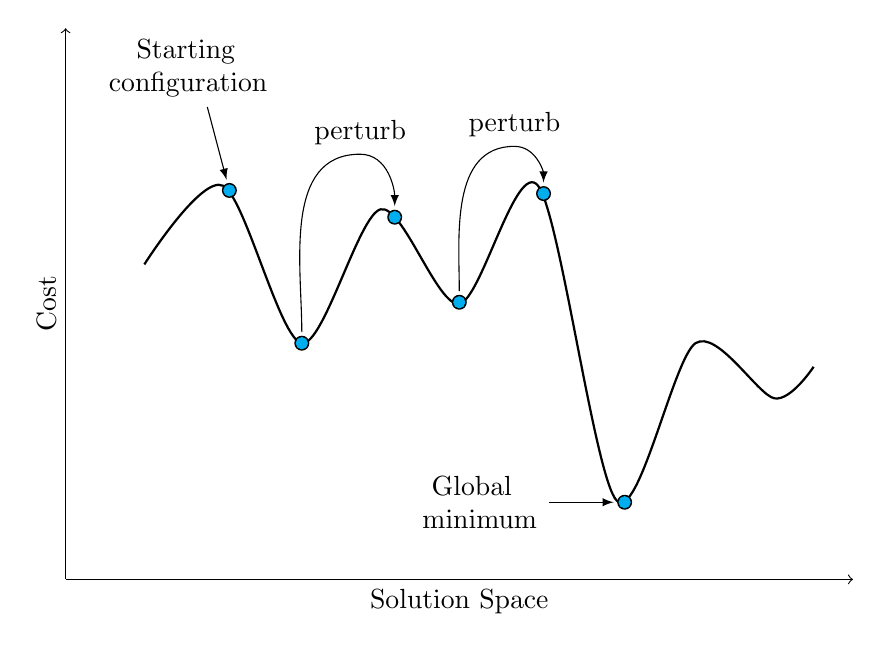
\begin{tikzpicture}[scale=1]
        \draw[->] (0,0) -- node[below] {Solution Space} (10,0);
        \draw[->] (0,0) -- node[above,sloped] {Cost} (0,7);
    
        \coordinate (A) at (1, 4);
        \coordinate (B) at (2, 5);
        \coordinate (C) at (3, 3);
        \coordinate (D) at (4, 4.7);
        \coordinate (E) at (5, 3.5);
        \coordinate (F) at (6, 5);
        \coordinate (G) at (7, 1);
        \coordinate (H) at (8, 3);
        \coordinate (I) at (9, 2.3);
        \coordinate (J) at (9.5, 2.7);
    
        \draw[black,thick] plot [smooth] coordinates {(A) (B) (C) (D) (E) (F) (G) (H) (I) (J)};
    
        \coordinate (P1) at (2.08,4.94);
        \coordinate (P2) at (3,3);
        \coordinate (P3) at (4.18,4.6);
        \coordinate (P4) at (5,3.52);
        \coordinate (P5) at (6.07,4.9);
        \coordinate (P6) at (7.1,0.98);

		\coordinate (P2_3) at (3.74,5.4);
		\coordinate (P4_5) at (5.7,5.5);

		\coordinate (SP) at (1.8,6);
		\coordinate (GB) at (6,0.98);
        
        % Draw jump arrows
        \draw[black,-latex,shorten <=4pt,shorten >=4pt] (P2) to[out=90, in=180] (P2_3) to[out=0, in=90] (P3);
        \node[above] at (P2_3) {perturb};
        \draw[black,-latex,shorten <=4pt,shorten >=4pt] (P4) to[out=90, in=180] (P4_5) to[out=0, in=90] (P5);
        \node[above] at  (P4_5) {perturb};
        
        % Comment arrows
        \draw[black,-latex,shorten >=4pt] (SP) -- (P1);
        \node[above,yshift=0,text width=25mm] at (SP) {\quad Starting \quad configuration};
        \draw[black,-latex,shorten <=4pt,shorten >=4pt] (GB) -- (P6);
        \node[left,xshift=13,yshift=0,text width=18mm] at (GB) {\ Global \ minimum};
        
    
        % Draw points
        \foreach \point in {P1,P2,P3,P4,P5,P6}  {
            \filldraw [black] (\point) circle (2.5pt);
            \filldraw [cyan] (\point) circle (2pt);
        }
    
    \end{tikzpicture}
    \caption{Iteration process of VNS}
    \label{fig:vns}
\end{figure}

% VNS balances exploration (through varying neighborhood structures) and exploitation (through local search) to efficiently search the solution space.
% The number of edges that we decide to swap can be dependent of the size of the instance, if we were working on a small instance, e.g. 
% ~50 nodes, swapping more than ten edges could result in a change way too big of the starting solution, worsening it unnecessarily.

\subsection{Perturbation implementation}

\begin{figure}[htbp]
    \textbf{Perturb} \\
    \begin{algorithm}[H]
        \SetKwInOut{Input}{Input}
        \SetKwInOut{Output}{Output}
        \Input{A tour $T$ of $G$ as an array of indices \newline Perturbation magnitude $p$}
        \Output{A perturbated tour $T_p$}
        \BlankLine
        $L \gets [\;]$\\
        \For{$i \in \{0,1,\dots,p-1\}$}{
            \BlankLine
            $r \gets $ random in range $[0,|T|)$\\
            \lWhile{$r \in L$}{$r \gets $ random in range $[0,|T|)$}
            $L \gets L \cup \{r\}$
        }
        \BlankLine
        $b \gets T[L[0]]$\\
        \BlankLine
        \For{$i \in \{0,1,\dots,p-2\}$}{
            \BlankLine
            $T[L[i]] \gets T[L[i+1]]$
        }
        \BlankLine
        $T[L[p-1]] \gets b$\\
        \BlankLine
        \Return $T$
    \end{algorithm}
    \caption{Perturbation procedure} \label{fig:vnsPerturbPseudocode}
\end{figure}

The \textbf{perturbation} is the procedure in which the solution is changed to escape the local minima.
It's very important to choose a suitable perturbation method for the selected local neighborhood search algorithm.
It has to be able to modify the solution enough to escape local optimal points while not modifying it too much as to land in a completely different state.

In the literature, the perturbation does not have a strict definition, instead it depends on the optimization problem and the local search method chosen while still retaining some freedom for its implementation.
Our implementation involves swapping nodes at random in the solution array.
The process consists in the following steps:
\begin{enumerate}
    \item Select a the permutation magnitude, which is the number of nodes that will change their position inside the solution array; this choice is made at random between a defined interval.
    \item Choose at random the nodes which will be affected by the perturbation, with particular care to not select the same element twice.
    \item According to the order in which nodes were selected for the perturbation, move them in a circular way between each other in the solution array.
\end{enumerate}

% \subsection{Implementation(? Maybe talk specifics on how kick works)}
% For the implementation of VNS we have the main function VariableNeighborhoodSearch which is in charge of managing the various threads initialization 
% and coordination, along with the time management in order to maintain the execution of the algorithm within the time limit provided in input.
% Inside the threads we will run parallely the function runVns, which performs the actual algorithm.
% The loop inside the threads will start by taking the passed solution and perform a repeating cycle of 2-opt operations and kicks. 2-opt is in charge 
% of searching the local space of the solution, while the kick will ensure a traslation to a neighboring search space.
% For the kick we implemented a swap of a dynamically chosen amount of edges. We did this to adapt to different scales of instances, since a fixed 
% amount of edges swaps (e.g. five each time) could result in a non-effective enough of a neighborhood change for large instances. All the edges involved in the kick are selected randomly.
% After each execution of 2-opt the obtained solution will be compared with the saved best solution found so far, and, if the cost is improved, the 
% best solution gets updated. Note that the best solution is shared among the threads and its access is managed by mutex.

\subsection{Performance}

Our implementation of VNS requires tuning only one hyperparameter: the perturbation magnitude interval.
Each time that we apply a perturbation a number within the interval is picked at random, and it represents the amount of nodes in the solution array that are getting swapped.

In order to find the best possible variable we tested the algorithm by running it in different configurations multiple times.
The intervals we chose to test were: [4,4], [5,5], [5,10], [5,20], [5,40] and [20,40].
As shown by \figurename{ \ref{fig:vnsParmTune}}, the best overall intervals were the [5,5] and the [5,10] with a slight advantage of the latter.

\begin{figure}[htbp]
	\centering
	\begin{tikzpicture}
        \begin{axis}[
            xlabel={Cost Ratio},
            xmin=1, xmax=1.015,
            ymin=0, ymax=74,
            xtick={1,1.005,1.01,1.015},
            xticklabel style={/pgf/number format/fixed,/pgf/number format/precision=4},
            ytick=\empty,
            legend style={at={(0.98,0.02)},anchor=south east,legend columns=1},
			legend cell align={left},
            xmajorgrids=true,
            grid style=dashed,
        ]
        
        \addplot[Blue,mark=square,mark size=1.5] table[x=p4_4cost, y=idx, col sep=semicolon] {csv/vns.csv}; 
        \addplot[Red,mark=o,mark size=1.5] table[x=p5_5cost, y=idx, col sep=semicolon] {csv/vns.csv};
        \addplot[Green,mark=triangle,mark size=1.5] table[x=p5_10cost, y=idx, col sep=semicolon] {csv/vns.csv};
        \addplot[Purple,mark=star,mark size=1.5] table[x=p5_20cost, y=idx, col sep=semicolon] {csv/vns.csv};
        \addplot[Dandelion,mark=otimes,mark size=1.5] table[x=p5_40cost, y=idx, col sep=semicolon] {csv/vns.csv};
        \addplot[Black,mark=diamond,mark size=1.5] table[x=p20_40cost, y=idx, col sep=semicolon] {csv/vns.csv};
        \addlegendentry{[ 4, 4]}
        \addlegendentry{[ 5, 5]}
        \addlegendentry{[ 5,10]}
        \addlegendentry{[ 5,20]}
        \addlegendentry{[ 5,40]}
        \addlegendentry{[20,40]}
            
        \end{axis}
    \end{tikzpicture}
	\caption{Performance comparison between different perturbation magnitude intervals} \label{fig:vnsParmTune}
\end{figure}

\begin{figure}[htbp]
	\centering
	\begin{tikzpicture}
        \begin{axis}[
            ylabel={Iterations/s Ratio},
            xlabel={Sorted instances},
            xmin=0, xmax=74,
            ymin=1, ymax=18,
            ytick={1,2,4,6,8,10,12,14,16},
            xtick=\empty,
            legend style={at={(0.02,0.98)},anchor=north west,,legend columns=1},
			legend cell align={left},
            ymajorgrids=true,
            grid style=dashed,
        ]
        
        \addplot[Blue,mark=square,mark size=1.5] table[y=p4_4iter, x=idx, col sep=semicolon] {csv/vns.csv}; 
        \addplot[Red,mark=o,mark size=1.5] table[y=p5_5iter, x=idx, col sep=semicolon] {csv/vns.csv};
        \addplot[Green,mark=triangle,mark size=1.5] table[y=p5_10iter, x=idx, col sep=semicolon] {csv/vns.csv};
        \addplot[Purple,mark=star,mark size=1.5] table[y=p5_20iter, x=idx, col sep=semicolon] {csv/vns.csv};
        \addplot[Dandelion,mark=otimes,mark size=1.5] table[y=p5_40iter, x=idx, col sep=semicolon] {csv/vns.csv};
        \addplot[Black,mark=diamond,mark size=1.5] table[y=p20_40iter, x=idx, col sep=semicolon] {csv/vns.csv};
        \addlegendentry{[ 4, 4]}
        \addlegendentry{[ 5, 5]}
        \addlegendentry{[ 5,10]}
        \addlegendentry{[ 5,20]}
        \addlegendentry{[ 5,40]}
        \addlegendentry{[20,40]}
            
        \end{axis}
    \end{tikzpicture}
	\caption{Comparison between VNS parameters in speed.} \label{fig:vnsIters}
\end{figure}

To investigate these differences in performance we also compared the speed that each configuration yielded.
\figurename{ \ref{fig:vnsIters}} highlights the large gap in speed between each of the selected intervals, with smaller intervals, and with smaller bounds, running faster compared to larger ones.
This behavior is to be expected since a higher perturbation magnitude causes solutions to be of overall worse quality compared to solutions affected by lighter perturbation.
Of course the higher the quality of a solution after a perturbation, the less time 2-Opt will take to optimize it, which explains the difference in speed between each configuration.

However there is likely more to this behavior than simple execution speed.
For istance, we can hypothesize that perturbations of a magnitude that is too high could be causing the algorithm to skip over high quality areas in solution space.
The opposite is true as well: a perturbation that isn't strong enough problably does not manage to escape local minima neighborhoods as it was the case with the [4,4] interval.

Likely, to find a good hyperparameter that can be of the right magnitude to both prevent skipping over the optimal solution neighborhood but still ensure escaping local minimas, a better criterion shoud be applied. 
%A way to obtain the best from both phenomemon likely lies in a different criterion in which the magnitude in picked inside the interval.
In our implementations we selected the size of the perturbation by picking an element in the chosen interval uniformly at random.
Switching from that to a different distribution, like an exponential distribution, would allow smaller perturbation to be performed more often than larger ones.
This could result in a behavior that is overall fast due to the smaller average size of perturbation, but still able to escape larger valleys in solution space using rare but large perturbations.

\begin{figure}[htbp]
	\centering
	\begin{tikzpicture}
        \begin{axis}[
            xlabel={Cost Ratio},
            xmin=1, xmax=1.082,
            ymin=0, ymax=74,
            xtick={},
            ytick=\empty,
            legend style={at={(0.98,0.02)},anchor=south east,legend columns=1},
			legend cell align={left},
            xmajorgrids=true,
            grid style=dashed,
        ]
        
        \addplot[Blue,mark=square,mark size=1.5] table[x=startcost,y=idx, col sep=semicolon] {csv/vns.csv}; 
        \addplot[Red,mark=o,mark size=1.5] table[x=finalcost,y=idx, col sep=semicolon] {csv/vns.csv};
        \addplot[Green,mark=triangle,mark size=1.5] table[x=optimalcost,y=idx, col sep=semicolon] {csv/vns.csv}; 
        \addlegendentry{Initial Cost} 
        \addlegendentry{Final Cost}
        \addlegendentry{Optimal Cost}
            
        \end{axis}
    \end{tikzpicture}
	\caption{Performance of with perturbation interval set to [5,10]} \label{fig:vnsCost}
\end{figure}


\newpage

\section{Simulated Annealing}

\begin{figure}[htbp]
    \centering
    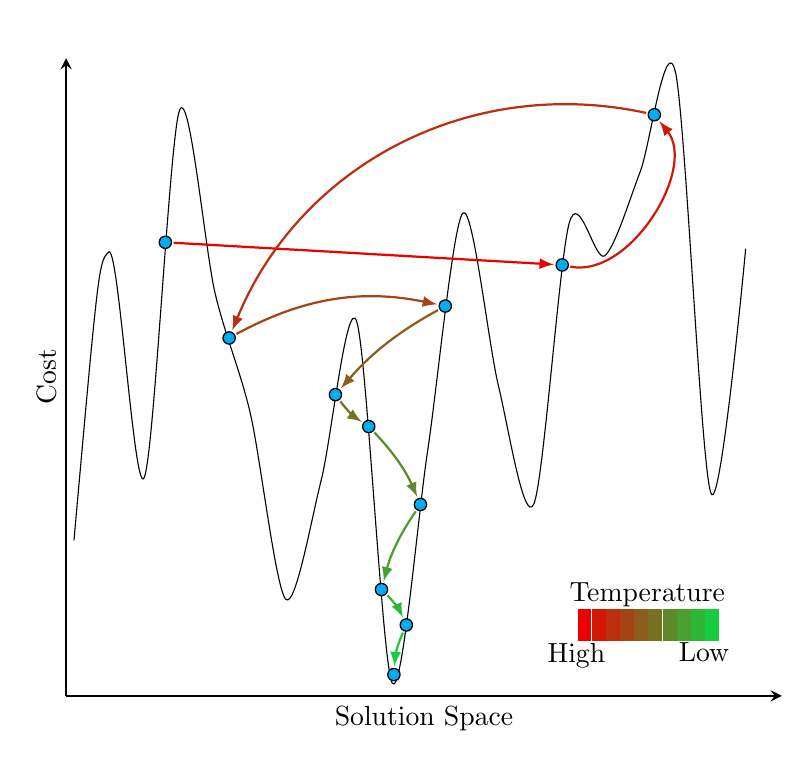
\begin{tikzpicture}
		[scale=0.9,shorten <=3pt,shorten >=3pt,>=stealth]

        \draw[thick,->,shorten <=0pt,shorten >=0pt,>=stealth] (-0.1,1) -- node[below] {Solution Space} (10,1);
        \draw[thick,->,shorten <=0pt,shorten >=0pt,>=stealth] (-0.1,1) -- node[above,sloped] {Cost} (-0.1,10);

		\draw[black,] plot [smooth] coordinates {(0,3.076)(0.5,7.263)(1,4.076)(1.5,9.263)(2,6.689)(2.5,4.981)(3,2.362)(3.5,4.046)(4,6.282)(4.5,1.183)(5,4.45)(5.5,7.813)(6,5.376)(6.5,3.708)(7,7.675)(7.5,7.209)(8,8.394)(8.5,9.791)(9,3.856)(9.5,7.428)};

        \coordinate (P1) at (1.3,7.4);
        \coordinate (P2) at (6.9,7.08);
        \coordinate (P3) at (8.2,9.2);
        \coordinate (P4) at (2.2,6.05);
        \coordinate (P5) at (5.25,6.5);
        \coordinate (P6) at (3.7,5.25);
        \coordinate (P7) at (4.17,4.8);
        \coordinate (P8) at (4.9,3.7);
        \coordinate (P9) at (4.35,2.5);
        \coordinate (P10) at (4.7,2);
        \coordinate (P11) at (4.525,1.3);
              
        \foreach \point in {P1,P2,P3,P4,P5,P6,P7,P8,P9,P10,P11}  {
            \filldraw [black] (\point) circle (2.5pt);
            \filldraw [cyan] (\point) circle (2pt);
        }

        \definecolor{C1}{RGB}{235, 0, 0}
        \definecolor{C2}{RGB}{211, 23, 7}
        \definecolor{C3}{RGB}{188, 46, 14}
        \definecolor{C4}{RGB}{164, 68, 20}
        \definecolor{C5}{RGB}{141, 91, 27}
        \definecolor{C6}{RGB}{118, 114, 34}
        \definecolor{C7}{RGB}{94, 137, 41}
        \definecolor{C8}{RGB}{71, 160, 48}
        \definecolor{C9}{RGB}{47, 182, 54}
        \definecolor{C10}{RGB}{24, 205, 61}

		\draw[-latex,color=C1,thick] (P1) to (P2);
		\draw[-latex,color=C2,thick] (P2) to[bend right=70] (P3);
		\draw[-latex,color=C3,thick] (P3) to[bend right=40] (P4);
		\draw[-latex,color=C4,thick] (P4) to[bend left=20] (P5);
		\draw[-latex,color=C5,thick] (P5) to[bend right=10] (P6);
		\draw[-latex,color=C6,thick] (P6) to[bend right=10] (P7);
		\draw[-latex,color=C7,thick] (P7) to[bend left=10] (P8);
		\draw[-latex,color=C8,thick] (P8) to[bend right=10] (P9);
		\draw[-latex,color=C9,thick] (P9) to[bend left=10] (P10);
		\draw[-latex,color=C10,thick] (P10) to[bend right=10] (P11);

        \draw[line width=4mm, color=C1] (7,2) -- ++(0.43,0);
        \draw[line width=4mm, color=C2] (7.2,2) -- ++(0.43,0);
        \draw[line width=4mm, color=C3] (7.4,2) -- ++(0.43,0);
        \draw[line width=4mm, color=C4] (7.6,2) -- ++(0.43,0);
        \draw[line width=4mm, color=C5] (7.8,2) -- ++(0.43,0);
        \draw[line width=4mm, color=C6] (8,2) -- ++(0.43,0);
        \draw[line width=4mm, color=C7] (8.2,2) -- ++(0.43,0);
        \draw[line width=4mm, color=C8] (8.4,2) -- ++(0.43,0);
        \draw[line width=4mm, color=C9] (8.6,2) -- ++(0.43,0);
        \draw[line width=4mm, color=C10] (8.8,2) -- ++(0.43,0);

        \node[above,yshift=3] at (8.1,2) {Temperature};
        \node[below,yshift=-3] at (7.1,2) {High};
        \node[below,yshift=-3] at (8.9,2) {Low};

    \end{tikzpicture}
    \caption{Iteration process of Simulated Annealing}
    \label{fig:sa}
\end{figure}

Simulated Annealing is a probabilistic metaheuristic inspired by the annealing process in metallurgy, where a material in heated and then slowly cooled in order to improve some of its traits.
The key parameter in this method is in fact called \textit{temperature}.
The value of this parameter indicates the rate for which we allow our method to accept swaps that have a positive offset\footnote{The concepts of swap and offset are the same as in the 2-Opt section}.
Initially this parameter is set high, which allows for a greater exploration of the solution space.
At every iteration this parameter is scaled down (by a factor of $0.9$ or $0.95$ for example), gradually avoiding swaps of too low quality, thus restricting the search space. 
This process is regulated to restart every time the temperature gets too low and there are no more swaps that are allowed due to the low temperature.

In our implementation we decided to perform more than one swap for each temperature value.
The number of swaps performed before updating the temperature is decided at complilation time.

Another key point in our implementation is the "forced cooling".
This technique consists in running 2-Opt whenever the randomized swap search isn't able to find a swap that is accepted given the current temperature value.
Such behavior is practically always triggered at low temperatures, when the solution is good enough that the randomized search isn't able to find good enough swaps to be accepted within an upper bound on the number of attempts.
We chose to set the number of nodes of the instance as attempts upper bound.

We also chose to implement two criteria describing the quality of swaps.
The chosen criteria determines a quality value which is compared againts the current annealing temperature: if the quality value is lower than the temperature then the swap is accepted\footnote{A swap is better the lower its quality indicator is}.

\textbf{Swap ratio acceptance (SRA)} is a criterion which evaluates a swap quality according to the ratio between the newly introduced edges and the replaced ones.
\[
    q = \frac{c(e^{new}_i) + c(e^{new}_j)}{c(e^{old}_{i'}) + c(e^{old}_{j'})}
\]
By construction, $q \in (\infty,0)$, where $q > 1$ means that the swap offset is positive, while $q < 1$ means the offset is negative.
This means that extra care must be put into the temperature cooldown effect, since at temperature lower than 1 even optimizing swaps can be rejected.
To fix this issue it's possible to either adjust the temperature formulation such that its lower bound becomes 1(asymptotical) or to just stop decreasing the temperature when it reaches one.
 
\textbf{Average cost ratio acceptance (ACRA)} evaluates instead the ratio between a swap offset and the average cost of edges in a solution.
\[
    q = \frac{\text{offset}(w)}{c(T)/|V|}
\]
where $w$ is refers to the swap, $c(T)$ is the cost of solution $T$ and $|V|$ is the number of nodes in the instance as well as the number of edges in $T$.
By construction, $q \in \Re$ and since $c(T)/|V| > 0$ than $sign(q) = sign(offset(w))$.
Therefore there are no issues in allowing the temperature value to reach 0.


% \subsection{Implementation}
% For the implementation of Simulated Annealing we decided to set up a number of constants in order to be able to tweak the parameters of the method in input.
% Fixed parameters can work fine for instances of similar magnitude, but to allow for a good execution for both large and small instances we thought this was the best approach.
% The parameteres we are talking are:
% \begin{enumerate}
%     \item SAME\_TEMP\_MOVES\_THRESHOLD: Number of moves to perform before reducing the temperature.
%     \item TEMPERATURE\_MULTIPLIER: Factor by which the temperature is multiplied to decrease it; should be slightly less than 1.
%     \item STOP\_TEMP: Temperature at which SA stops and runs a 2-opt algorithm for further optimization.
%     \item MAX\_TRIES\_FUNC(n): Function to determine the maximum number of move attempts before increasing the temperature.
%     \item USE\_RATIO\_ACCEPTANCE: A macro to toggle the use of ratio-based acceptance criteria.
% \end{enumerate}
% The execution of this metaheuristic is managed by the function SimulatedAnnealing, that mainly sets up the desired number of threads and launches them 
% on the function runSimulatedAnnealing. 
% The actual algorithm is then executed parallely within each thread until the time limit is reached. During this time we perform moves up to what we 
% specified on STOP\_TEMP, then we will launch the 2-opt metaheuristic to further refine the solution within its space. 
% After a certain amount of non-improving iterations, we restart the method from the best solution found so far, which we are keeping track at all 
% times and is accessible by the use of a mutex by all threads. This is to fully use the time provided in the time limit, and to give the method more chances to escape a local minima.

\subsection{Performance}

When gathering the data to measure the performance of Simulated Annealing we encountered some issues.
In some instances of the TSP, the cost would not improve, regardless the temperature and criterion used.
Another anormality we detected regared the independence between the final solution cost and all tunable parameters.

\begin{figure}[htbp]
	\centering
	\begin{tikzpicture}
        \begin{axis}[
            xlabel={Cost Ratio},
            xmin=1, xmax=1.01,
            ymin=0, ymax=69,
            xtick={},
            xticklabel style={/pgf/number format/fixed,/pgf/number format/precision=4},
            ytick=\empty,
            legend style={at={(0.98,0.02)},anchor=south east,legend columns=1},
			legend cell align={left},
            xmajorgrids=true,
            grid style=dashed,
        ]
        
        \addplot[Blue,mark=square,mark size=1.5] table[x=ACRA-3, y=idx, col sep=semicolon] {csv/annealing.csv}; 
        \addplot[Red,mark=o,mark size=1.5] table[x=ACRA-6, y=idx, col sep=semicolon] {csv/annealing.csv};
        \addplot[Green,mark=triangle,mark size=1.5] table[x=ACRA-9, y=idx, col sep=semicolon] {csv/annealing.csv};
        \addplot[Purple,mark=star,mark size=1.5] table[x=SRA-3, y=idx, col sep=semicolon] {csv/annealing.csv};
        \addplot[Dandelion,mark=otimes,mark size=1.5] table[x=SRA-6, y=idx, col sep=semicolon] {csv/annealing.csv};
        \addplot[Black,mark=diamond,mark size=1.5] table[x=SRA-9, y=idx, col sep=semicolon] {csv/annealing.csv};
        \addlegendentry{$10^3$ ACRA}
        \addlegendentry{$10^6$ ACRA}
        \addlegendentry{$10^9$ ACRA}
        \addlegendentry{$10^3$ SRA}
        \addlegendentry{$10^6$ SRA}
        \addlegendentry{$10^9$ SRA}
            
        \end{axis}
    \end{tikzpicture}
	\caption{Performance comparison between different Simulated Annealing configurations in terms of $\frac{final\_cost}{start\_cost}$}
    \label{fig:annealingParmTune}
\end{figure}

\begin{figure}[htbp]
	\centering
	\begin{tikzpicture}
        \begin{axis}[
            ylabel={Iterations/s Ratio},
            xlabel={Sorted instances},
            xmin=0, xmax=69,
            ymin=1, ymax=2.5,
            ytick={},
            xtick=\empty,
            legend style={at={(0.02,0.98)},anchor=north west,,legend columns=1},
			legend cell align={left},
            ymajorgrids=true,
            grid style=dashed,
        ]
        
        
        \addplot[Blue,mark=square,mark size=1.5] table[y=ACRA-3-iter, x=idx, col sep=semicolon] {csv/annealing.csv}; 
        \addplot[Red,mark=o,mark size=1.5] table[y=ACRA-6-iter, x=idx, col sep=semicolon] {csv/annealing.csv};
        \addplot[Green,mark=triangle,mark size=1.5] table[y=ACRA-9-iter, x=idx, col sep=semicolon] {csv/annealing.csv};
        \addplot[Purple,mark=star,mark size=1.5] table[y=SRA-3-iter, x=idx, col sep=semicolon] {csv/annealing.csv};
        \addplot[Dandelion,mark=otimes,mark size=1.5] table[y=SRA-6-iter, x=idx, col sep=semicolon] {csv/annealing.csv};
        \addplot[Black,mark=diamond,mark size=1.5] table[y=SRA-9-iter, x=idx, col sep=semicolon] {csv/annealing.csv};
        \addlegendentry{$10^3$ ACRA}
        \addlegendentry{$10^6$ ACRA}
        \addlegendentry{$10^9$ ACRA}
        \addlegendentry{$10^3$ SRA}
        \addlegendentry{$10^6$ SRA}
        \addlegendentry{$10^9$ SRA}
            
        \end{axis}
    \end{tikzpicture}
	\caption{Comparison between Simulated Annealing parameters in speed}
    \label{fig:annealingIters}
\end{figure}

\figurename{ \ref{fig:annealingParmTune}} shows exactly the second issue, picturing a too small difference between all results, even when considering instances with different size.

As for the previous algorithms, we also compared the speed in which each setting performed, discovering that even in those there isn't a drammatic enough difference to explain the anormalities.

To properly explain this behavior we would require much more time compared to other algorithms, like NN or VNS, since not only there are parameters to tune, but we must also consider the different quality criteria used.

Since there doesn't seems to be any particular configuration which allows for a better performance we arbitrarely chose the ACRA with temperature set to $10^6$ to compare this algorithm with the best solutions as well as the other algorithms later on.

\begin{figure}[htbp]
	\centering
	\begin{tikzpicture}
        \begin{axis}[
            xlabel={Cost Ratio},
            xmin=1, xmax=1.082,
            ymin=0, ymax=69,
            xtick={},
            ytick=\empty,
            legend style={at={(0.98,0.02)},anchor=south east,legend columns=1},
			legend cell align={left},
            xmajorgrids=true,
            grid style=dashed,
        ]
        
        \addplot[Blue,mark=square,mark size=1.5] table[x=startcost,y=idx, col sep=semicolon] {csv/annealing.csv}; 
        \addplot[Red,mark=o,mark size=1.5] table[x=finalcost,y=idx, col sep=semicolon] {csv/annealing.csv};
        \addplot[Green,mark=triangle,mark size=1.5] table[x=optimalcost,y=idx, col sep=semicolon] {csv/annealing.csv}; 
        \addlegendentry{Initial Cost} 
        \addlegendentry{Final Cost}
        \addlegendentry{Optimal Cost}
            
        \end{axis}
    \end{tikzpicture}
	\caption{Overall Performance of Simulated Annealing using ACRA with temperature set to $10^6$.}
    \label{fig:annealingCost}
\end{figure}

As shown by \figurename{ \ref{fig:annealingCost}}, Simulated Annealing manages to find the best solution, altough this happens only in small instances.
A detail which is not perceptible from the comparison is that often Simulated Annealing completely fails to find any sort of improvement to the starting solution, ending its computation with the same exact solution as it started with.

\newpage

\section{Genetic}

Genetic Algorithms (GAs), pioneered by John Holland in the 1960s, represent a significant innovation in the field of optimization.
They draw inspiration from the principles of natural selection and genetics.
By simulating processes such as selection, crossover, and mutation on a population of potential solutions, GAs iteratively evolve towards optimal or near-optimal solutions.
Their ability to efficiently navigate large and complex search spaces has led to their application across diverse domains, including engineering, economics, and artificial intelligence.
%The robustness and versatility of GAs make them a powerful tool for tackling problems with expansive, poorly understood search spaces.

In TSP case, Genetic Algorithms are particularly useful due to the complexity and enormity of the solution space.
GAs approach this by encoding each possible route (solution) as a chromosome.

The process begins with a population of these chromosomes, which then undergo selection based on their fitness; typically, the shorter the route, the higher the fitness.
New offspring solutions are then generated through crossover, which combines segments from two parent solutions.
Mutation introduces diversity by randomly altering parts of a solution, helping to avoid premature convergence on local optima.
Additionally, new chromosomes can be periodically introduced in each generation to increase variety.

Over successive generations, the GA refines the population, ideally converging on the shortest route.
The flexibility of GAs in handling various constraints and large search spaces makes them a robust choice for solving TSP and similar optimization problems.

\subsection{Implementation}

Aside from the usual iterative part which runs the algorithm over multiple iterations (or generations), this metaheuristic can be divided into smaller subrutines.

\subsubsection{Cromosome introduction/generation}

The first generation that GA works upon is, in our case, a set of \textbf{completely randomly generated permutation}.
With random permutation we mean that, starting from any random valid solution of a TSP instance, the generation procedure simply applies some random permutation on the order in which the nodes are visited.
Therefore, given enough permuations, it creates a chromosome very different from the starting one.
This very same procedure is adopted when introducing new chromosomes in the population.
Altough not the best in term of producing good solutions, it still represent a very quick and easy way to generate new diverse solutions.

\subsubsection{Crossover}

The crossover part is likely the iconic and most characteristic part of GA algorithms.
There are many different methods used to merge two chromosomes into an offspring and, most of the time, they are task specific.
In the TSP case, a lot of operators capable of performing such merge have been developed.

We chose the \textbf{edge recombination operator} (\textbf{ERO}).
The idea behind ERO involves the construction of a merged adiacency matrix from the parents.
Then, starting from a random node, a successor is chosen based on the number of neighbors it has in the merged adiacency matrix or at random when the candidate nodes have the same number of neighbors.
At every iteration the successor is added to the offspring and it is than removed from the all the neighborhoods inside the adiacency matrix.
This process is repeated util the merged adiacency matrix is empty and the offspring solution is complete.

\subsubsection{Mutation}

Mutation is another tactic used in GAs to increase the variability of the results.
In our case we implemented two types of mutation:
\begin{itemize}
    \item \textbf{Node swap} consists in simply swapping two nodes in the solution, effectively changing four edges.
    \item \textbf{Edge swap} is a random swap of the same kind used in 2-Opt, without regarding the quality of the swap in any way.
\end{itemize}

It's easy to see how using our GA implementation without introducing new solutions from permutations and crossover results in an algorithm that is somewhat similar to SA.

\subsection{Performance}

\begin{itemize}
    \item \textbf{Config 1}: Population = 50, Crossover = 10, Mutation = 10, Reintro =  5
    \item \textbf{Config 2}: Population = 50, Crossover = 20, Mutation = 20, Reintro =  5
    \item \textbf{Config 3}: Population = 100, Crossover = 50, Mutation = 20, Reintro = 20
    \item \textbf{Config 4}: Population = 100, Crossover = 20, Mutation = 50, Reintro = 20
    \item \textbf{Config 5}: Population = 100, Crossover = 40, Mutation = 40, Reintro = 10
\end{itemize}

\begin{figure}[H]
	\centering
	\begin{tikzpicture}
        \begin{axis}[
            xlabel={Cost Ratio},
            xmin=1, xmax=2.7,
            ymin=0, ymax=42,
            xtick={},
            xticklabel style={/pgf/number format/fixed,/pgf/number format/precision=4},
            ytick=\empty,
            legend style={at={(0.98,0.02)},anchor=south east,legend columns=1},
			legend cell align={left},
            xmajorgrids=true,
            grid style=dashed,
        ]
        
        \addplot[Blue,mark=square,mark size=1.5] table[x=cost_50_10_10_5, y=idx, col sep=semicolon] {csv/genetic.csv}; 
        \addplot[Red,mark=o,mark size=1.5] table[x=cost_50_20_20_5, y=idx, col sep=semicolon] {csv/genetic.csv};
        \addplot[Green,mark=triangle,mark size=1.5] table[x=cost_100_50_20_20, y=idx, col sep=semicolon] {csv/genetic.csv};
        \addplot[Purple,mark=star,mark size=1.5] table[x=cost_100_20_50_20, y=idx, col sep=semicolon] {csv/genetic.csv};
        \addplot[Dandelion,mark=otimes,mark size=1.5] table[x=cost_100_40_40_10, y=idx, col sep=semicolon] {csv/genetic.csv};
        \addlegendentry{Config 1}
        \addlegendentry{Config 2}
        \addlegendentry{Config 3}
        \addlegendentry{Config 4}
        \addlegendentry{Config 5}
            
        \end{axis}
    \end{tikzpicture}
	\caption{Performance comparison between different Genetic configurations}
    \label{fig:geneticParmTune}
\end{figure}

\begin{figure}[H]
	\centering
	\begin{tikzpicture}
        \begin{axis}[
            ylabel={Iterations/s Ratio},
            xlabel={Sorted instances},
            xmin=0, xmax=42,
            ymin=1, ymax=8,
            ytick={},
            xtick=\empty,
            legend style={at={(0.02,0.98)},anchor=north west,,legend columns=1},
			legend cell align={left},
            ymajorgrids=true,
            %xmajorgrids=true,
            grid style=dashed,
        ]
        
        
        \addplot[Blue,mark=square,mark size=1.5] table[y=iter_50_10_10_5, x=idx, col sep=semicolon] {csv/genetic.csv}; 
        \addplot[Red,mark=o,mark size=1.5] table[y=iter_50_20_20_5, x=idx, col sep=semicolon] {csv/genetic.csv};
        \addplot[Green,mark=triangle,mark size=1.5] table[y=iter_100_50_20_20, x=idx, col sep=semicolon] {csv/genetic.csv};
        \addplot[Purple,mark=star,mark size=1.5] table[y=iter_100_20_50_20, x=idx, col sep=semicolon] {csv/genetic.csv};
        \addplot[Dandelion,mark=otimes,mark size=1.5] table[y=iter_100_40_40_10, x=idx, col sep=semicolon] {csv/genetic.csv};
        \addlegendentry{Config 1}
        \addlegendentry{Config 2}
        \addlegendentry{Config 3}
        \addlegendentry{Config 4}
        \addlegendentry{Config 5}
            
        \end{axis}
    \end{tikzpicture}
	\caption{Comparison between Genetic configurations in speed}
    \label{fig:geneticIters}
\end{figure}

\begin{figure}[H]
	\centering
	\begin{tikzpicture}
        \begin{axis}[
            xlabel={Cost Ratio},
            xmin=1, xmax=17,
            ymin=0, ymax=42,
            xtick={},
            ytick=\empty,
            legend style={at={(0.98,0.02)},anchor=south east,legend columns=1},
			legend cell align={left},
            xmajorgrids=true,
            grid style=dashed,
        ]
        
        \addplot[Red,mark=o,mark size=1.5] table[x=finalcost,y=idx, col sep=semicolon] {csv/genetic.csv}; 
        \addplot[Green,mark=triangle,mark size=1.5] table[x=optimalcost,y=idx, col sep=semicolon] {csv/genetic.csv};
        \addlegendentry{Final Cost}
        \addlegendentry{Optimal Cost}
            
        \end{axis}
    \end{tikzpicture}
	\caption{Overall Performance of Genetic}
    \label{fig:geneticCost}
\end{figure}

\section{Comparison}

\begin{figure}[H]
	\centering
	\begin{tikzpicture}
        \begin{axis}[
            xlabel={Cost Ratio},
            %ylabel={Iterations/s Ratio},
            xmin=1, xmax=1.05,
            ymin=0, ymax=74,
            xtick={},
            xticklabel style={/pgf/number format/fixed,/pgf/number format/precision=4},
            ytick=\empty,
            legend style={at={(0.98,0.02)},anchor=south east,legend columns=1},
			legend cell align={left},
            %ymajorgrids=true,
            xmajorgrids=true,
            grid style=dashed,
        ]
        
        \addplot[Blue,mark=square,mark size=1.5] table[x=tabu_1, y=idx, col sep=semicolon] {csv/cmp_metaheuristics.csv}; 
        \addplot[Red,mark=o,mark size=1.5] table[x=vns_5-10, y=idx, col sep=semicolon] {csv/cmp_metaheuristics.csv};
        \addplot[Green,mark=triangle,mark size=1.5] table[x=annealing_std6, y=annealing_idx, col sep=semicolon] {csv/cmp_metaheuristics.csv};
        % \addplot[Purple,mark=star,mark size=1.5] table[x=genetic, y=genetic_idx, col sep=semicolon] {csv/cmp_metaheuristics.csv};
        \addlegendentry{tabu}
        \addlegendentry{VNS}
        \addlegendentry{Annealing}
        % \addlegendentry{Genetic}
            
        \end{axis}
    \end{tikzpicture}
	\caption{Comparsion between all metaheuristics with best parameters found}
    \label{fig:metacmp}
\end{figure}